\section{Design}

\subsection{Functional Requirements}
This is a list of key required features needed for this project to be successful.

\begin{figure}[H]
\caption{Functional requirements}
\begin{table}[H]
\begin{tabular}{|p{0.2\textwidth}|p{0.7\textwidth}|p{0.1\textwidth}|}
\hline
Feature                         & Function                                                                                                                                                        & Priority \\ \hline
Copyright smart contract        & Immutable code on a public ledger “blockchain“ for the purpose of establishing ownership or the copyright to a piece of work.                                   & CORE     \\ \hline
Multi-party distribution        & The ability to establish a complex ownership structure of multiple individuals/groups, all these owners will have equal ownership of the copyrighted work.      & CORE     \\ \hline
Ownership transfer              & The ability to change the ownership of a copyright from one complex structure to another with consent of all current owner(s).                                  & CORE     \\ \hline
Work verification               & Verification of a work to establish its originality with a reasonable accuracy for the platform, no duplicate works will be allowed to be registered.           & CORE     \\ \hline
Dispute filing                  & Allow any user to dispute a copyright with sufficient evidence and provide an option for resolving these disputes by the owner(s).                              & CORE     \\ \hline
Digital signing                 & Digitally sign a registered work with unique data that identifies it as original copyright registered, much like the traditional copyright registration symbol. & CORE     \\ \hline
Decentralised Work CDN \& proxy & Store registered works on a decentralised technology providing a free and open option for creators.                                                             & EXTRA    \\ \hline
Websocket updates               & Real-time updates for the front-end UI to provide a better end-user experience.                                                                                 & EXTRA    \\ \hline
\end{tabular}
\end{table}
\end{figure}

\subsection{Smart contract}

\subsubsection{Inspiration}

To design a smart contract without prior experience I decided to look at an existing contract and because I knew my contract was going to exhibit similar functionality and principles as \textbf{NFTs} I started with the EIP\footnote{\inlineQ{Ethereum Improvement Proposals (EIPs) describe standards for the Ethereum platform, including core protocol specifications, client APIs, and contract standards.}{eip}} for non-fungible tokens \nft. 

This describes a standard interface for all external methods and events \textbf{NFT} contracts need to implement, most are self-explanatory like balanceOf, ownerOf, transferFrom and the Transfer event. Then there's a methods concerning "approval" which is \keyword{Ethereum} speak for access control, essentially what addresses are allowed to transact with a token.

Interfaces are useful for understanding how the contract interacts with the outside world but not the internal working. So I found an implementation \href{https://github.com/OpenZeppelin/openzeppelin-contracts/blob/master/contracts/token/ERC721/ERC721.sol}{here} written by \href{https://github.com/OpenZeppelin}{OpenZeppelin} to gain an understanding of the internal operation.

\begin{figure}[H]
\caption{\href{https://github.com/OpenZeppelin/openzeppelin-contracts/blob/master/contracts/token/ERC721/ERC721.sol}{ERC721.sol} data mappings}
\centering
\begin{lstlisting}[language=Solidity]
// Mapping from token ID to owner 
mapping(uint256 => address) private _owners;

// Mapping owner address to token count
mapping(address => uint256) private _balances;

// Mapping from token ID to approved address
mapping(uint256 => address) private _tokenApprovals;

// Mapping from owner to operator approvals
mapping(address => mapping(address => bool)) private _operatorApprovals;
\end{lstlisting}
\end{figure}

This snippet is taken from the OpenZeppelin contract and is essentially how an \textbf{NFT} "works". a series of mappings that are saved in storage\footnote{storage is an area of the \keyword{EVM} that every smart contract has access to for storing state variables that need to persistent. memory and stack are also available} and are hash-maps from one type to another. \textit{\_owners} points to an address based on the input token id (uint256) all methods in the contract simply modify these mappings for example when you register a token your wallet address is saved in the map entry for the next id.

\subsubsection{Ownership structure}

This architecture was used as foundations for my new contract, however there is one major requirement of my system not supported by the \nft standard which is multi party ownership of a token. This alone wasn't going to represent copyright as works can quite often involve multiple people collaborating, the book I mentioned at the beginning of this report\cite{blockchain_revolution} has two authors, a system not representing the work and effort of all involved is not acceptable.

\begin{figure}[H]
\caption{Structured Ownership essential mappings}
\centering
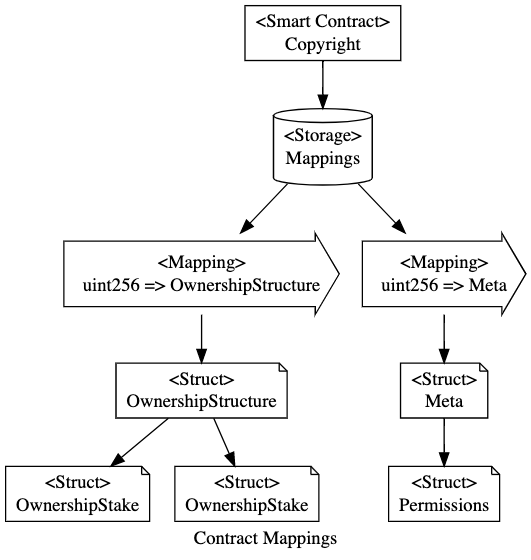
\includegraphics[width=0.5\textwidth,height=0.5\textheight,keepaspectratio]{images/operational/mappings.png}
\label{fig:float}
\end{figure}

To solve this problem I've redesigned how ownership is defined in the contract, instead of mapping token ids to one address the contract now maps to an \textbf{OwnershipStructure} that contains a list of owners along with a number of shares that specific address holds in the token. This design clearly borrows from limited companies share structure allowing a complex ownership of multiple individuals or groups with implied variance in ownership\footnote{Although the number of shares an address owns makes no immediate difference in the current implementation of this contract as this was outside of the desired complexity scope.}.

\subsubsection{Shareholder consensus}

Allowing multiple wallets to own a token now introduces a new problem for contract design, when a change is made everyone has to agree just check if you're an owner is not enough anymore, allowing everyone with a stake to make changes without consulting all other owners is a point of exploitation in need of solution.

\begin{figure}[H]
\caption{Structured Ownership proposal mappings}
\centering
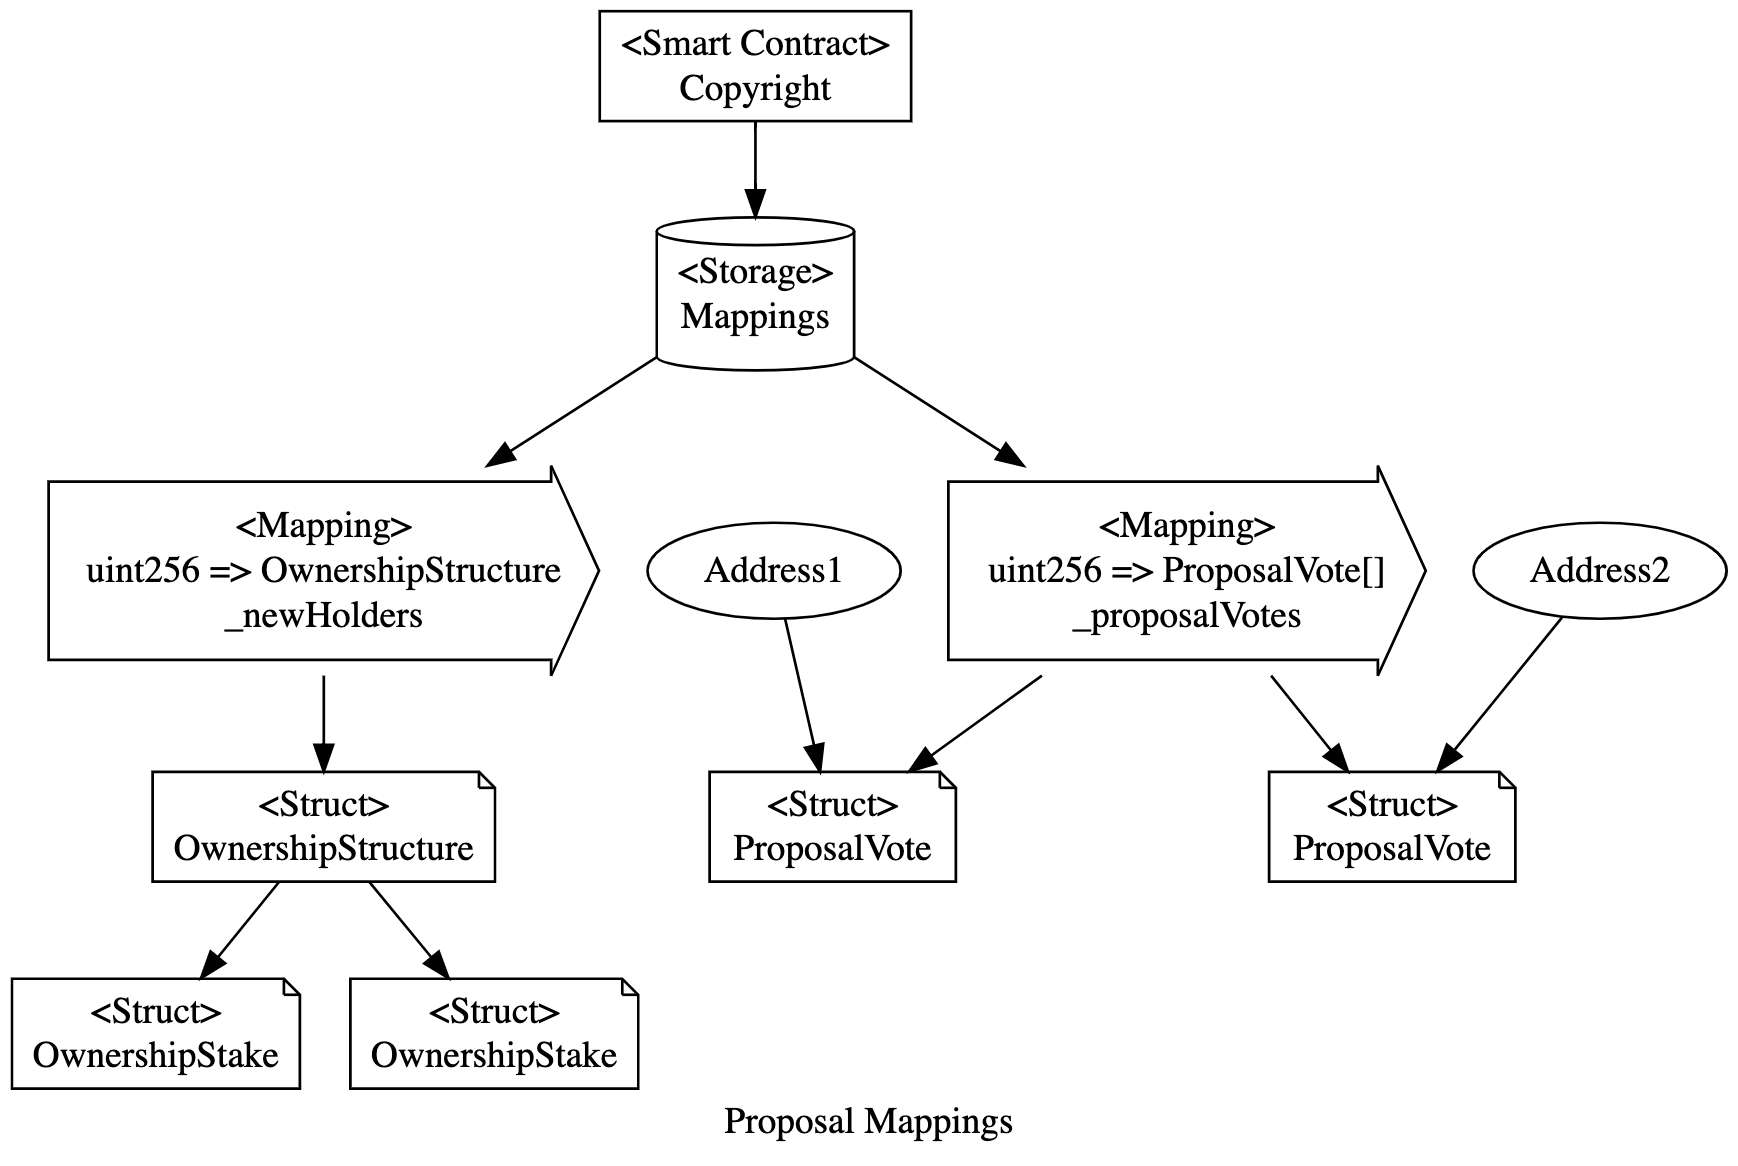
\includegraphics[width=\textwidth,height=\textheight,keepaspectratio]{images/operational/prop-mappings.png}
\end{figure}

I've designed this solution for the shareholder consensus problem, now instead of making direct changes to a copyright (above is an ownership restructure) a user proposes change to a copyright which is then voted on by all owners until a unanimous vote is reached then the change is made.

\subsubsection{Protections}

To simplify and give users customisability of protection I've designed a protections system similar to permission in many computer systems, the list of available protections was built from existing legal protections provided by \keyword{copyright} law \cite{rights_granted} including: Adaptation, Performance, Reproduction and Distribution. 

\subsection{Back-end}

\begin{figure}[H]
\caption{Back-end abstract operation}
\centering
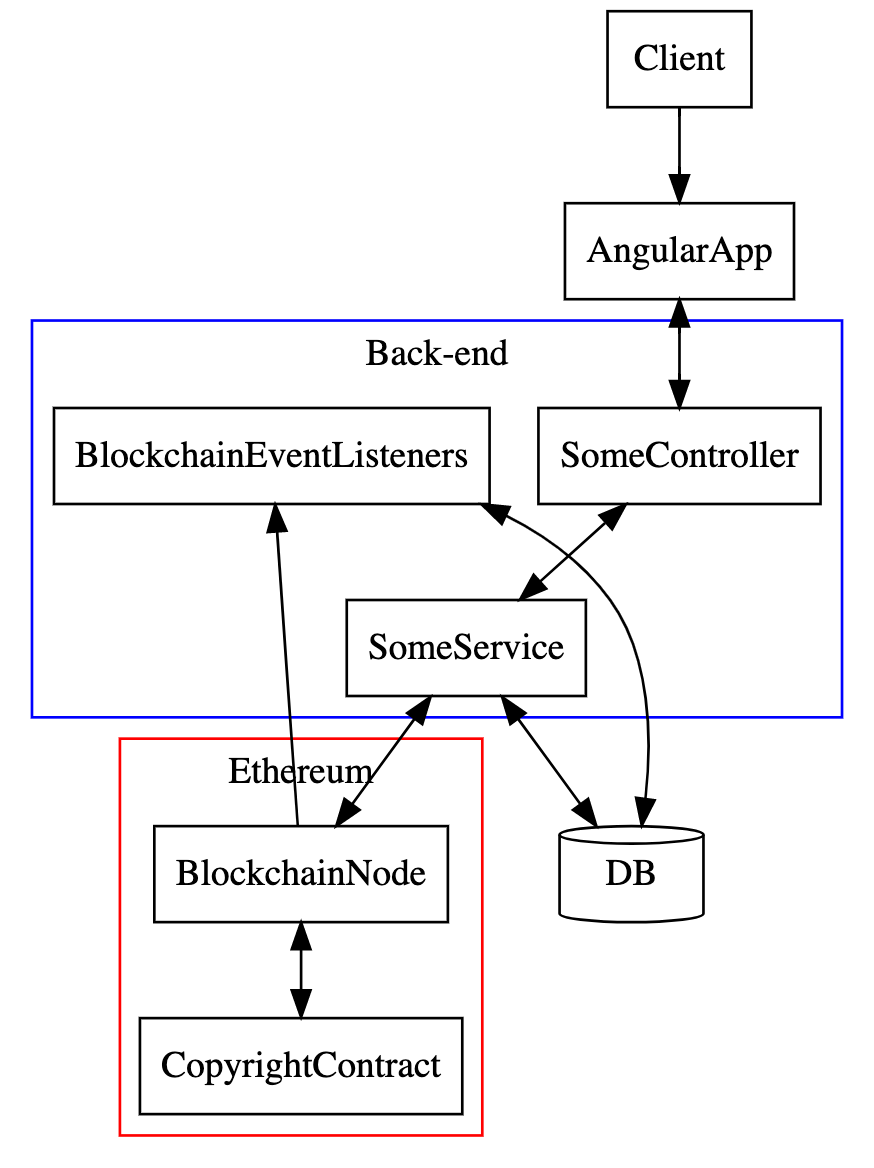
\includegraphics[width=\textwidth,height=0.4\textheight,keepaspectratio]{images/operational/example-backend}
\centering
\end{figure}

\subsubsection{Dependancy injection}

Dependancy injection is a supported and encouraged design pattern within \textbf{.NET} and \textbf{ASP.NET} which allows building loosely coupled applications by separating implementation and design, depending on a softwares design opposed to its technical implementation results in more resilient and modular code.

\begin{figure}[H]
\caption{DI graph taken from \href{https://docs.microsoft.com/en-us/dotnet/architecture/modern-web-apps-azure/architectural-principles#dependency-inversion}{docs.microsoft}}
\centering
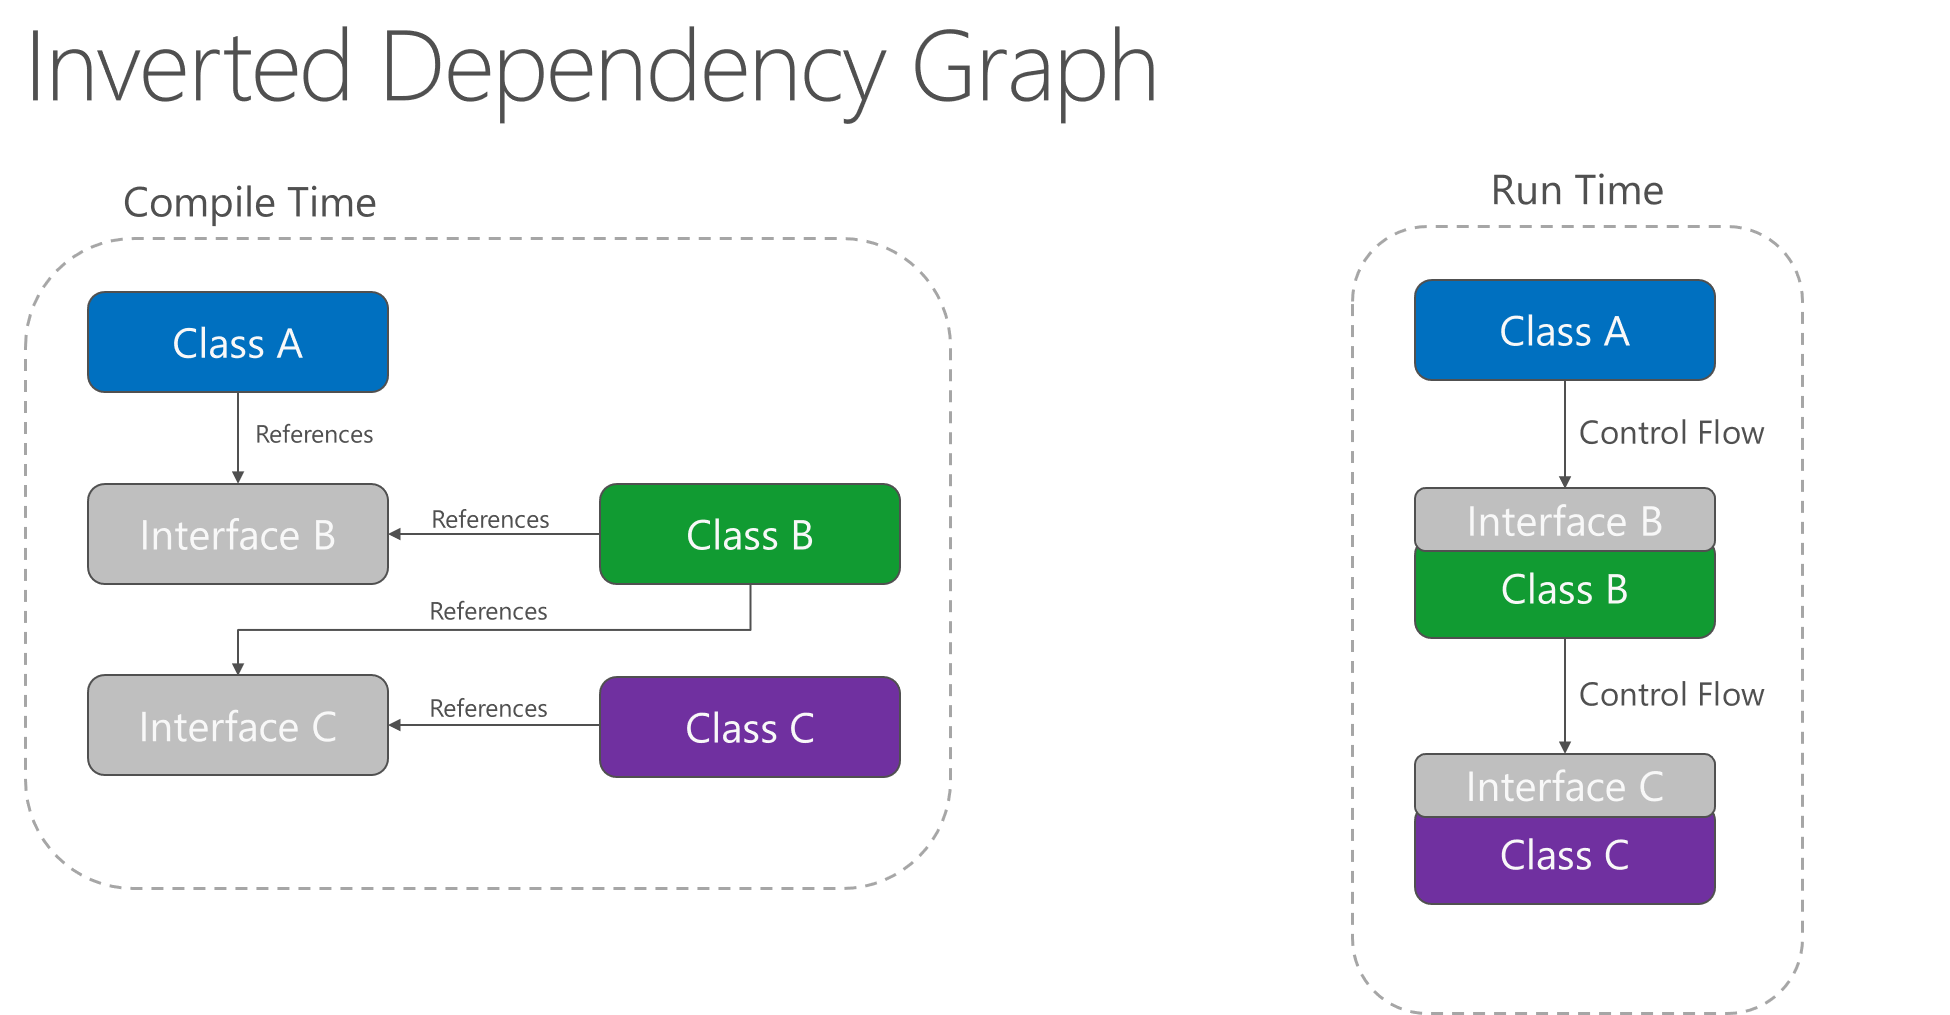
\includegraphics[width=\textwidth,height=\textheight,keepaspectratio]{images/patterns/ms-di}
\centering
\end{figure}

Above is an inversion of control and dependancy injection example, as you can see each class is depending on an interface of the desired class not the actual code implementation hence loosely coupled.

\begin{figure}[H]
\caption{Example dependancy graph for the query controller and service}
\centering
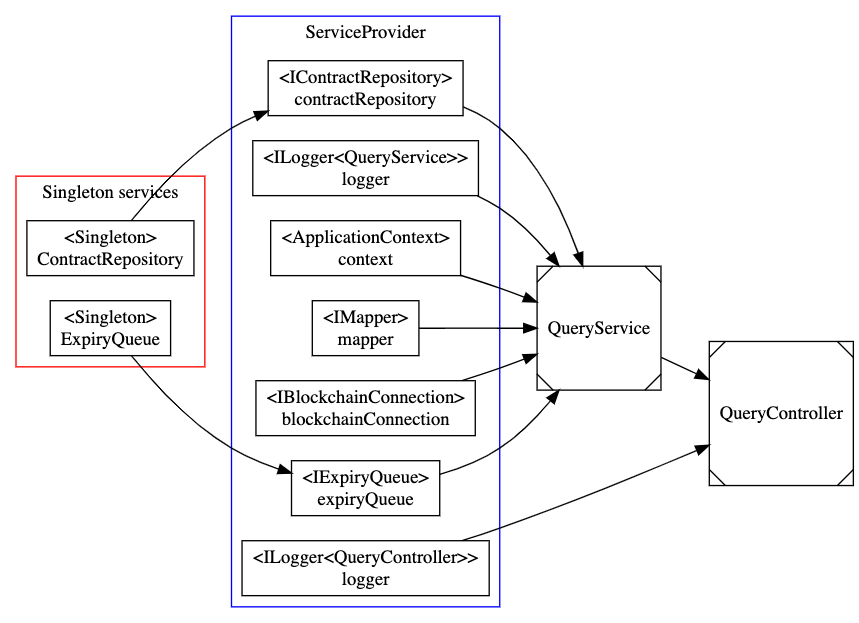
\includegraphics[width=0.7\textwidth,height=0.7\textheight,keepaspectratio]{images/patterns/DI-example}
\end{figure}

This is real example of dependancy injection drawn from the query controller and service injections. It shows both don't depend on any implemented classes just the interfaces which describe how you can interact with an implemented version of that class. At runtime each interface injected will be populated from the service collection with a real class that was registered on startup.

\subsubsection{Background services}

Background services was designed based on previous work I wrote for \href{https://github.com/mrharrisonbarker/openevent}{OpenEvent} so instead of using new software like \href{https://www.hangfire.io/}{Hangfire} which is more feature rich with a strong following I decided for the scale of this project and the existing pattern I had developed and knew intimately a year ago would be a better fit.

\begin{figure}[H]
\caption{Queued background service pattern}
\centering
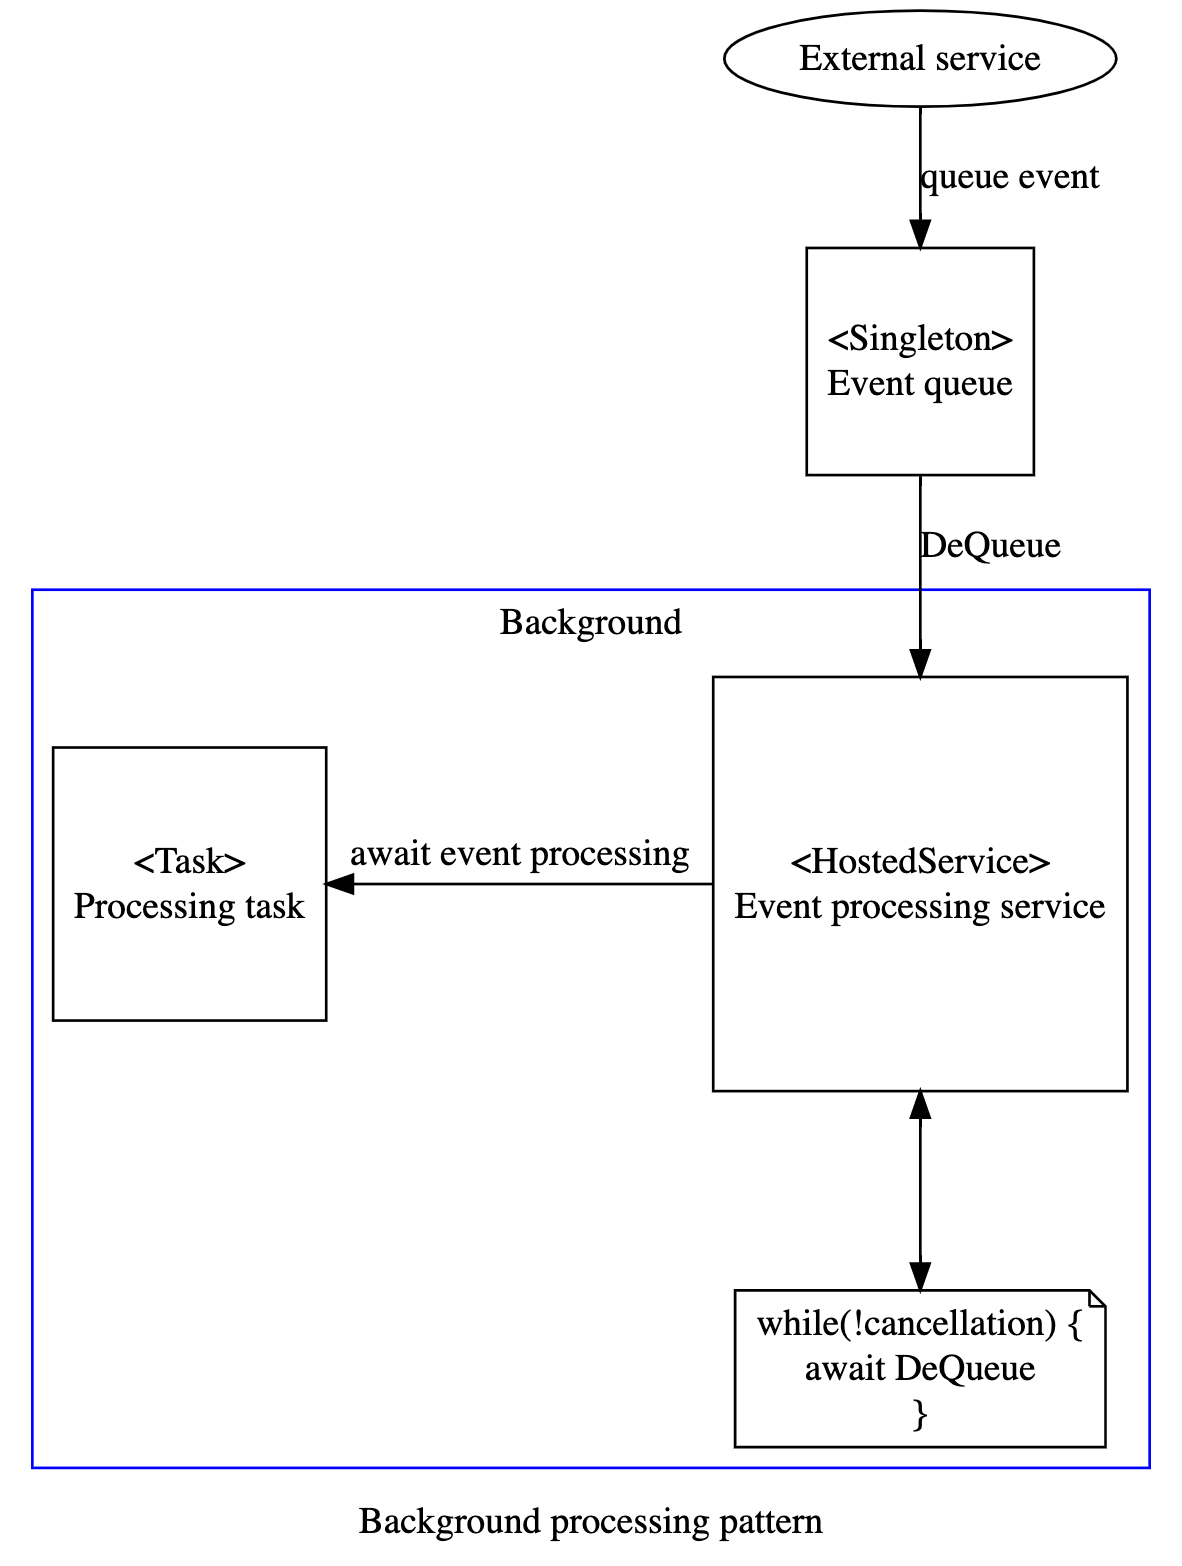
\includegraphics[width=0.5\textwidth,height=0.5\textheight,keepaspectratio]{images/patterns/background-processing-pattern}
\end{figure}

This is the basic pattern describing how my background services work, it's essentially a queue and processing service. `Work' is queued while a processing service running in its own thread dequeues work and processes, after this work completes the processing service waits for the next item to dequeue.

This pattern can be quickly implemented and tailored to specific background work, it's easily scalable with the number of threads configurable in the processing service.

\subsubsection{Event processing}

Because transactions on the \keyword{blockchain} can take any amount of time to be verified, placed into a block and for that block to be placed onto the chain. Blocks on \keyword{Ethereum} are processed around every 13 seconds but you're not guaranteed to be placed into the next block, this largely depends on the amount of \textbf{gas} you're willing to spend and the volume of current transactions.

All this means that my system must be able to send a transaction then wait an indeterminate amount of time for a response meaning I can't force the user to wait on that transaction until complete. Thankfully \keyword{Ethereum} has a solution for this  called \textbf{Events}, I've specified a number of these events in my contract (see below) which the back-end "listens" for by processing the information in each block.

\begin{figure}[H]
\caption{\href{https://github.com/MrHarrisonBarker/CRPL/blob/main/CRPL.Contracts/contracts/IStructuredOwnership.sol}{IStructuredOwnership} events}
\begin{lstlisting}[language=Solidity]
/// @dev Emits when a new copyright is registered
event Registered(uint256 indexed rightId, OwnershipStake[] to);

/// @dev Emits when a copyright has been restructured and bound
event Restructured(uint256 indexed rightId, RestructureProposal proposal);

/// @dev Emits when a restructure is proposed
event ProposedRestructure(uint256 indexed rightId, RestructureProposal proposal);

/// @dev Emits when a restructure vote fails
event FailedProposal(uint256 indexed rightId);
\end{lstlisting}
\end{figure}

When an event is found it gets added to a processing queue then a processing service dequeues each event and processes based on the type of event.

\begin{figure}[H]
\caption{Blockchain event listeners and processing}
\centering
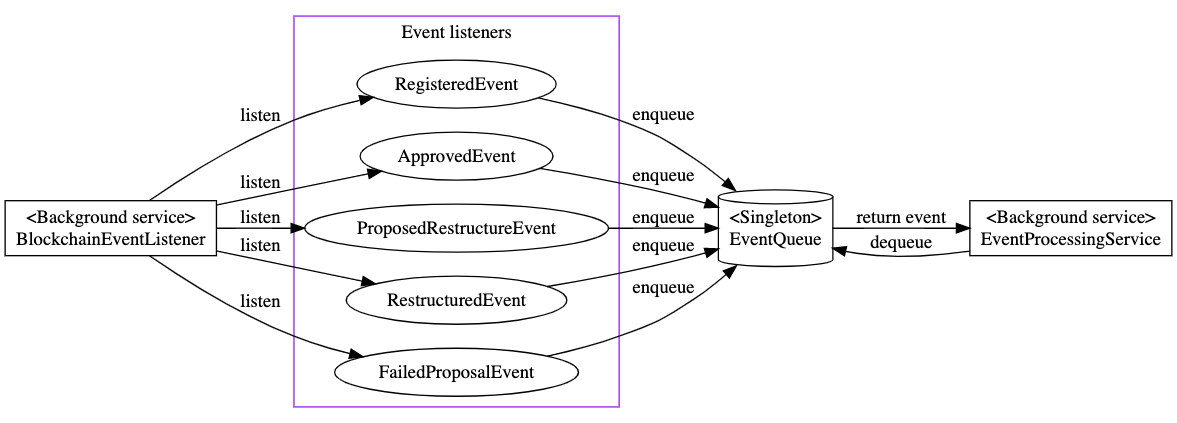
\includegraphics[width=\textwidth,height=0.5\textheight,keepaspectratio]{images/operational/Event-Listening}
\end{figure}

\subsubsection{Applications framework}

Handling forms and applications is awkward and full of edge cases, the code for handing these applications (eg: copyright registration) can become large and convoluted especially when your system implements many. For this system five applications are needed: copyright registration, ownership restructure, dispute, wallet transfer and delete account. I decided to design a solution for handling application flow and state as a generic process, this means all applications will follow the same state flow and interaction endpoints \textit{seen below.} 

\begin{figure}[H]
\caption{Applications framework state diagram}
\centering
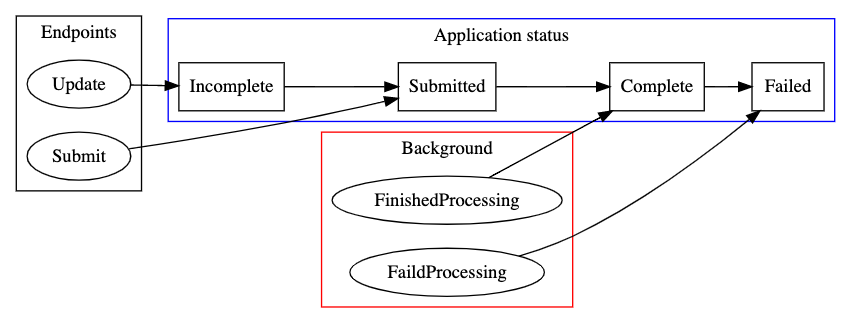
\includegraphics[width=\textwidth,height=0.5\textheight,keepaspectratio]{images/operational/applications-status}
\end{figure}

% TODO could probably so somewhere else
This generification and ridged design flow proved extremely useful, this was because keeping a clear view of state is essential when keeping parity between my system and the outer \keyword{blockchain}.

\subsection{Database}

The database needs to store two types of data: data stored on both the \keyword{blockchain} and CRPL (eg: public wallet addresses, contract address, and registered works) and data stored solely on the database not mirrored with the chain (eg: applications, user account information and explicit database relationships).

\begin{figure}[H]
\caption{Final database EER diagram}
\centering
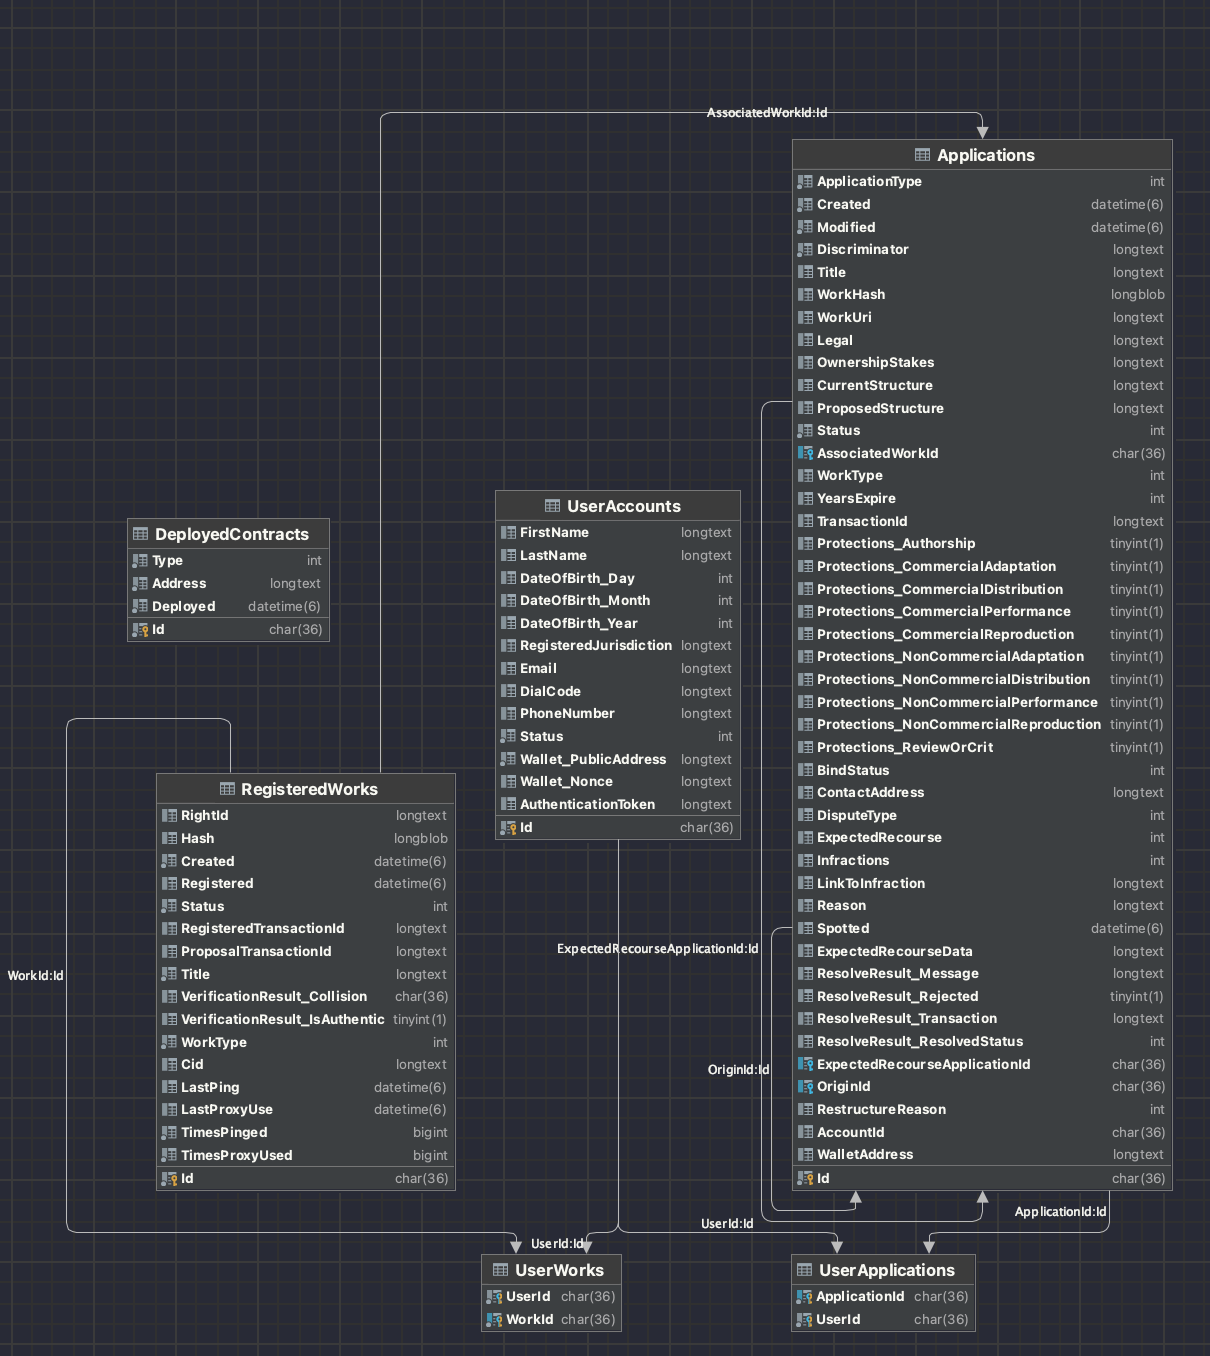
\includegraphics[width=\textwidth,height=0.7\textheight,keepaspectratio]{images/patterns/database}
\end{figure}

\subsubsection{Chain parity}
\label{sec:chain-parity}

Some data needs to be kept in parity with the \keyword{blockchain} this introduces a problem because data on the chain can change independently from the system, a user could transact with the \keyword{smart contract} and register a new copyright or propose a new ownership structure and even bind that new structure destroying any continuity between the database and what's real. This will lead to a terrible user experience but I can stop it, the chain is open to anyone and is the entire point of this project.

However I can react to change, everything is open and accessible all I have to do is read the \keyword{blockchain} and update the database accordingly keeping in mind the chain is always the source of truth not the database.

\subsubsection{Independent from the chain}

I've chosen to keep certain data off the \keyword{blockchain} only representing in the database. It's possible to store everything on chain completely independent of any database, however this would ballon the size of my \keyword{smart contract} which are limited to 24KB complied it would also hamper maintainability and future development.

Imagine everything is represented on the \keyword{smart contract} including dispute handling and applications, the contract is deployed on the chain and now running in the \keyword{EVM} what happens when I want to add a new type of application or discover my dispute handling is un-ethical or exploitable? I can't change the smart contract it's immutable, the only solution is deploy a new contract and manually migrate all previous \keyword{copyrights}, however this would be expensive, slow and arguably against the spirit of \keyword{blockchain} technology and the law as I'm effectively changing the underlying representation of a \keyword{copyright} without consultation or approval.

\subsection{Front-end}

Visual design of the web application was on lowest priority so a focus on pure usability and function was the goal because of the complex undertaking needed to implement all functionality building effectively two backend systems (\keyword{blockchain} and web API).

I decided to use the \href{https://clarity.design/}{Clarity} design system and libraries as they have support for Angular with an enterprise/function first focus.

\begin{figure}[H]
\caption{Original dashboard page wireframe}
\centering
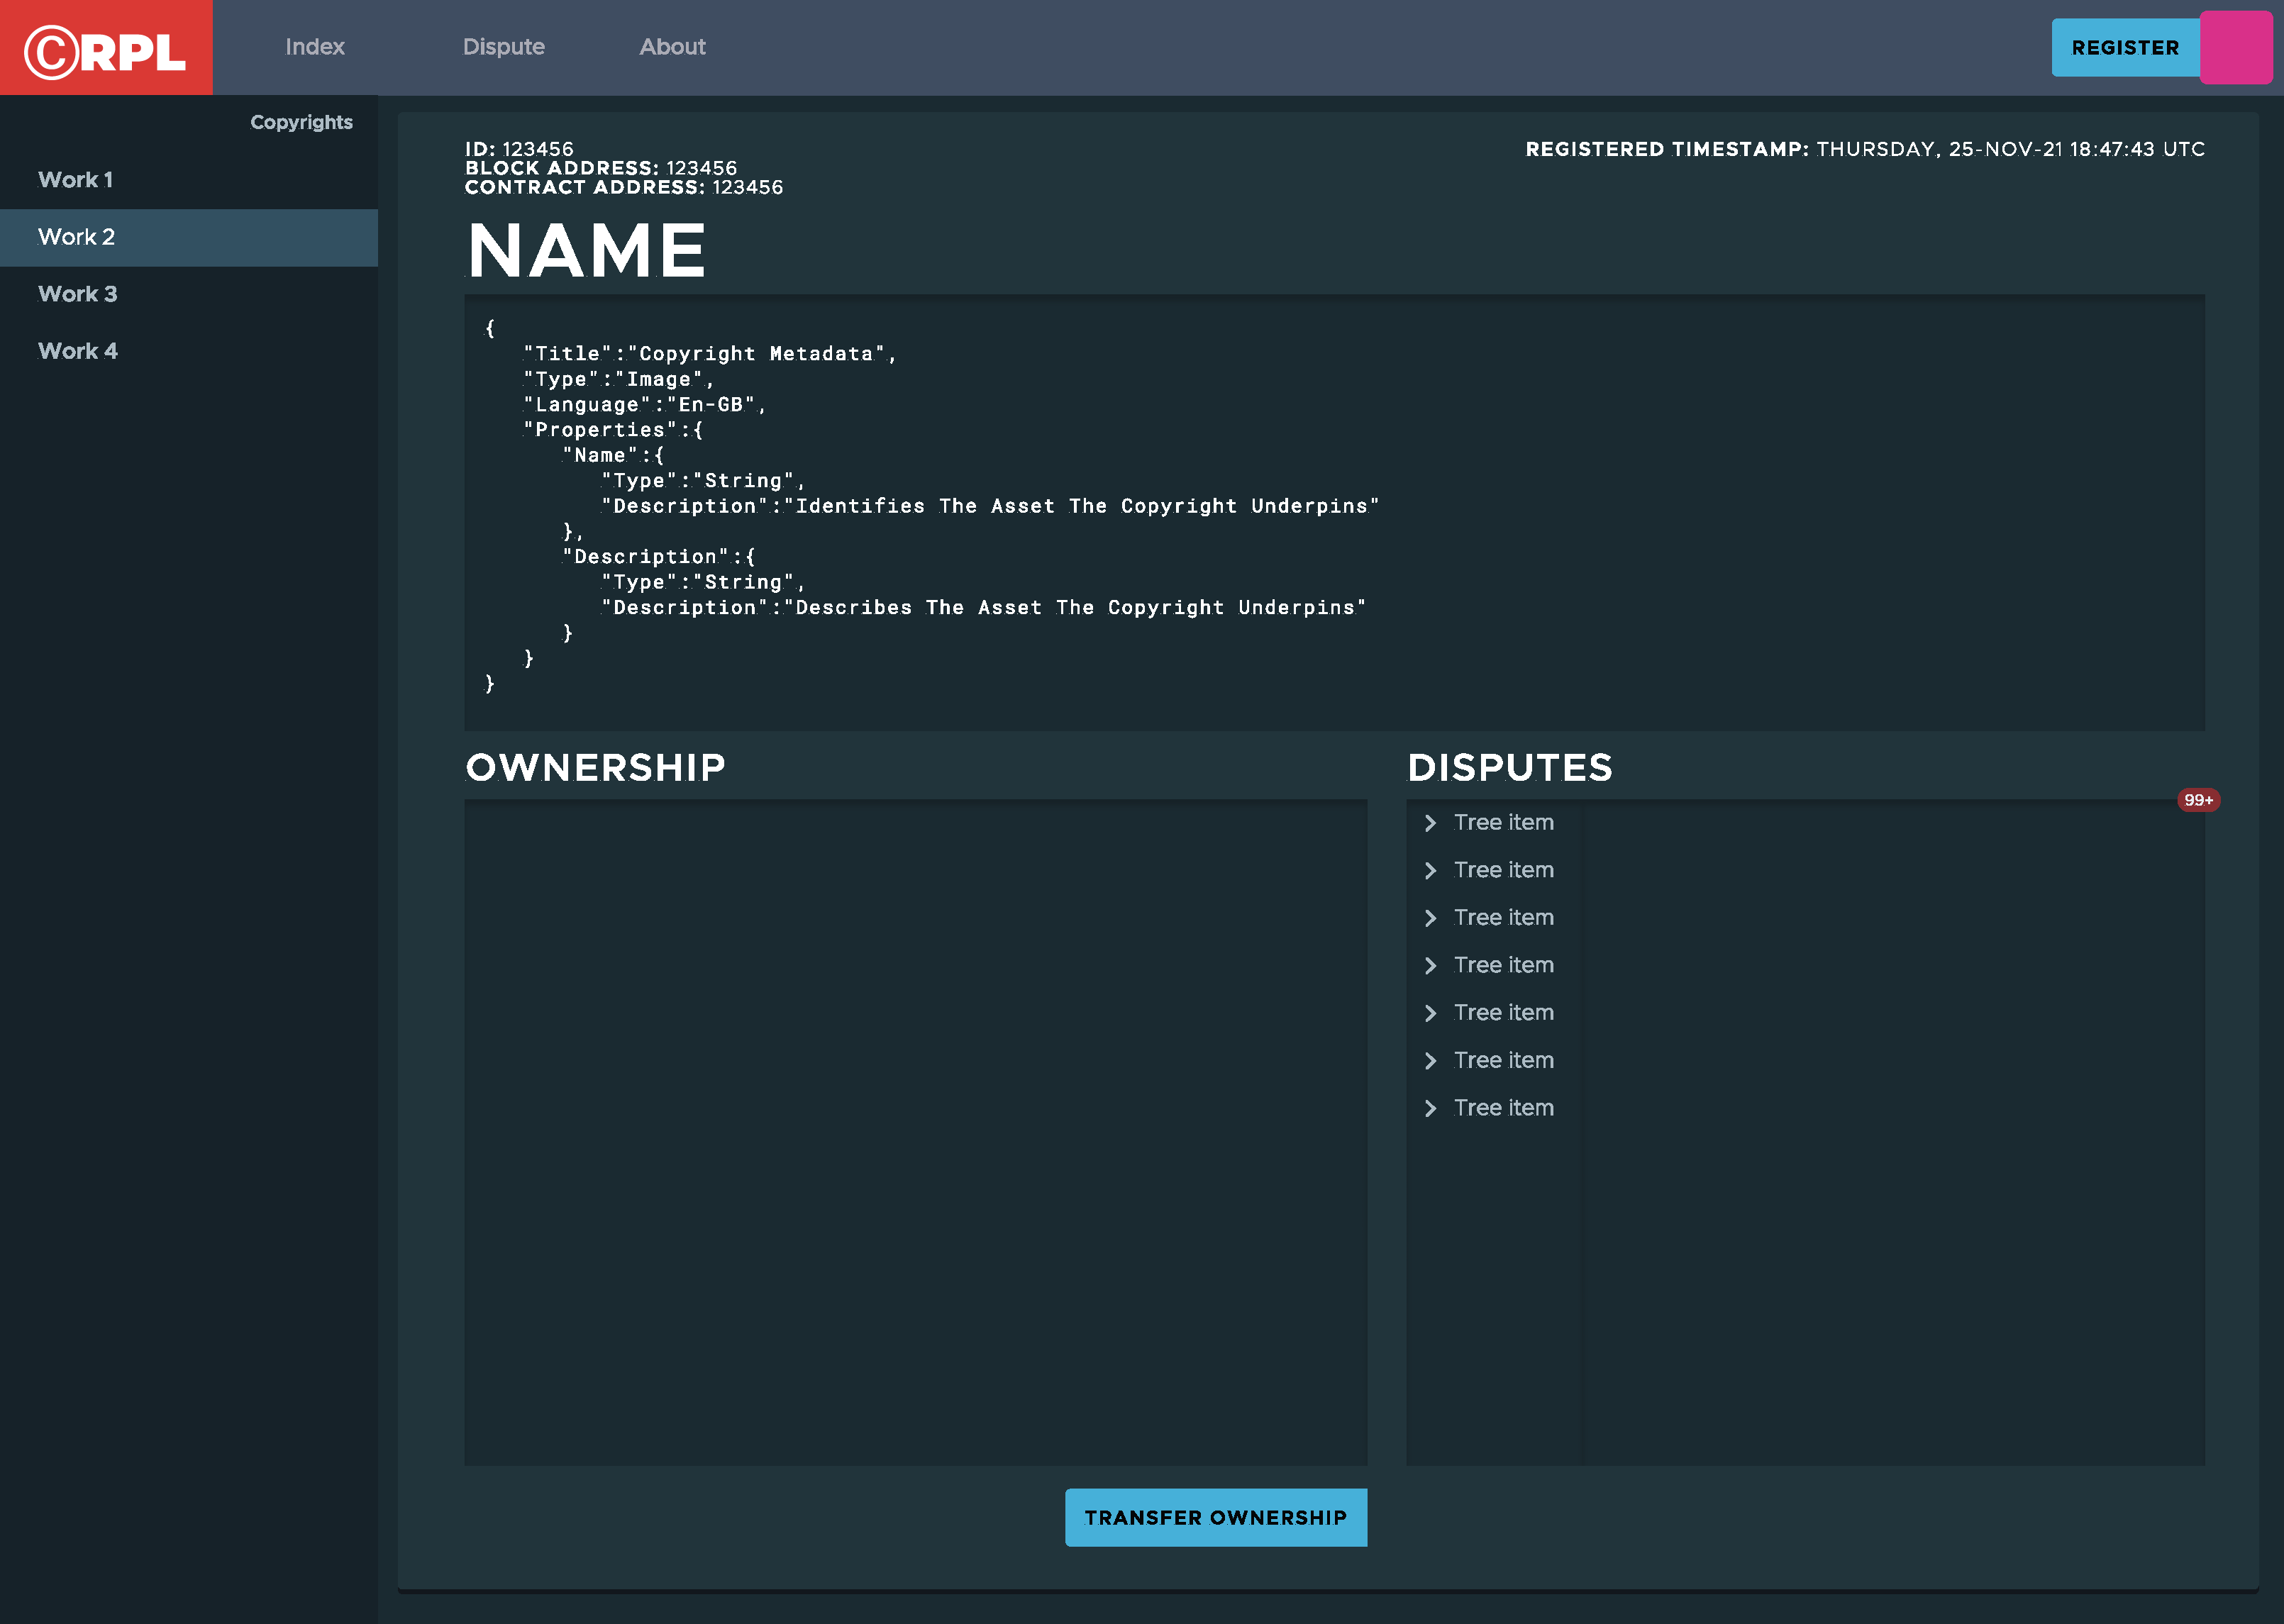
\includegraphics[width=\textwidth,height=0.5\textheight,keepaspectratio]{images/wireframe/Dashboard}
\end{figure}

\begin{figure}[H]
\caption{Final dashboard design}
\centering
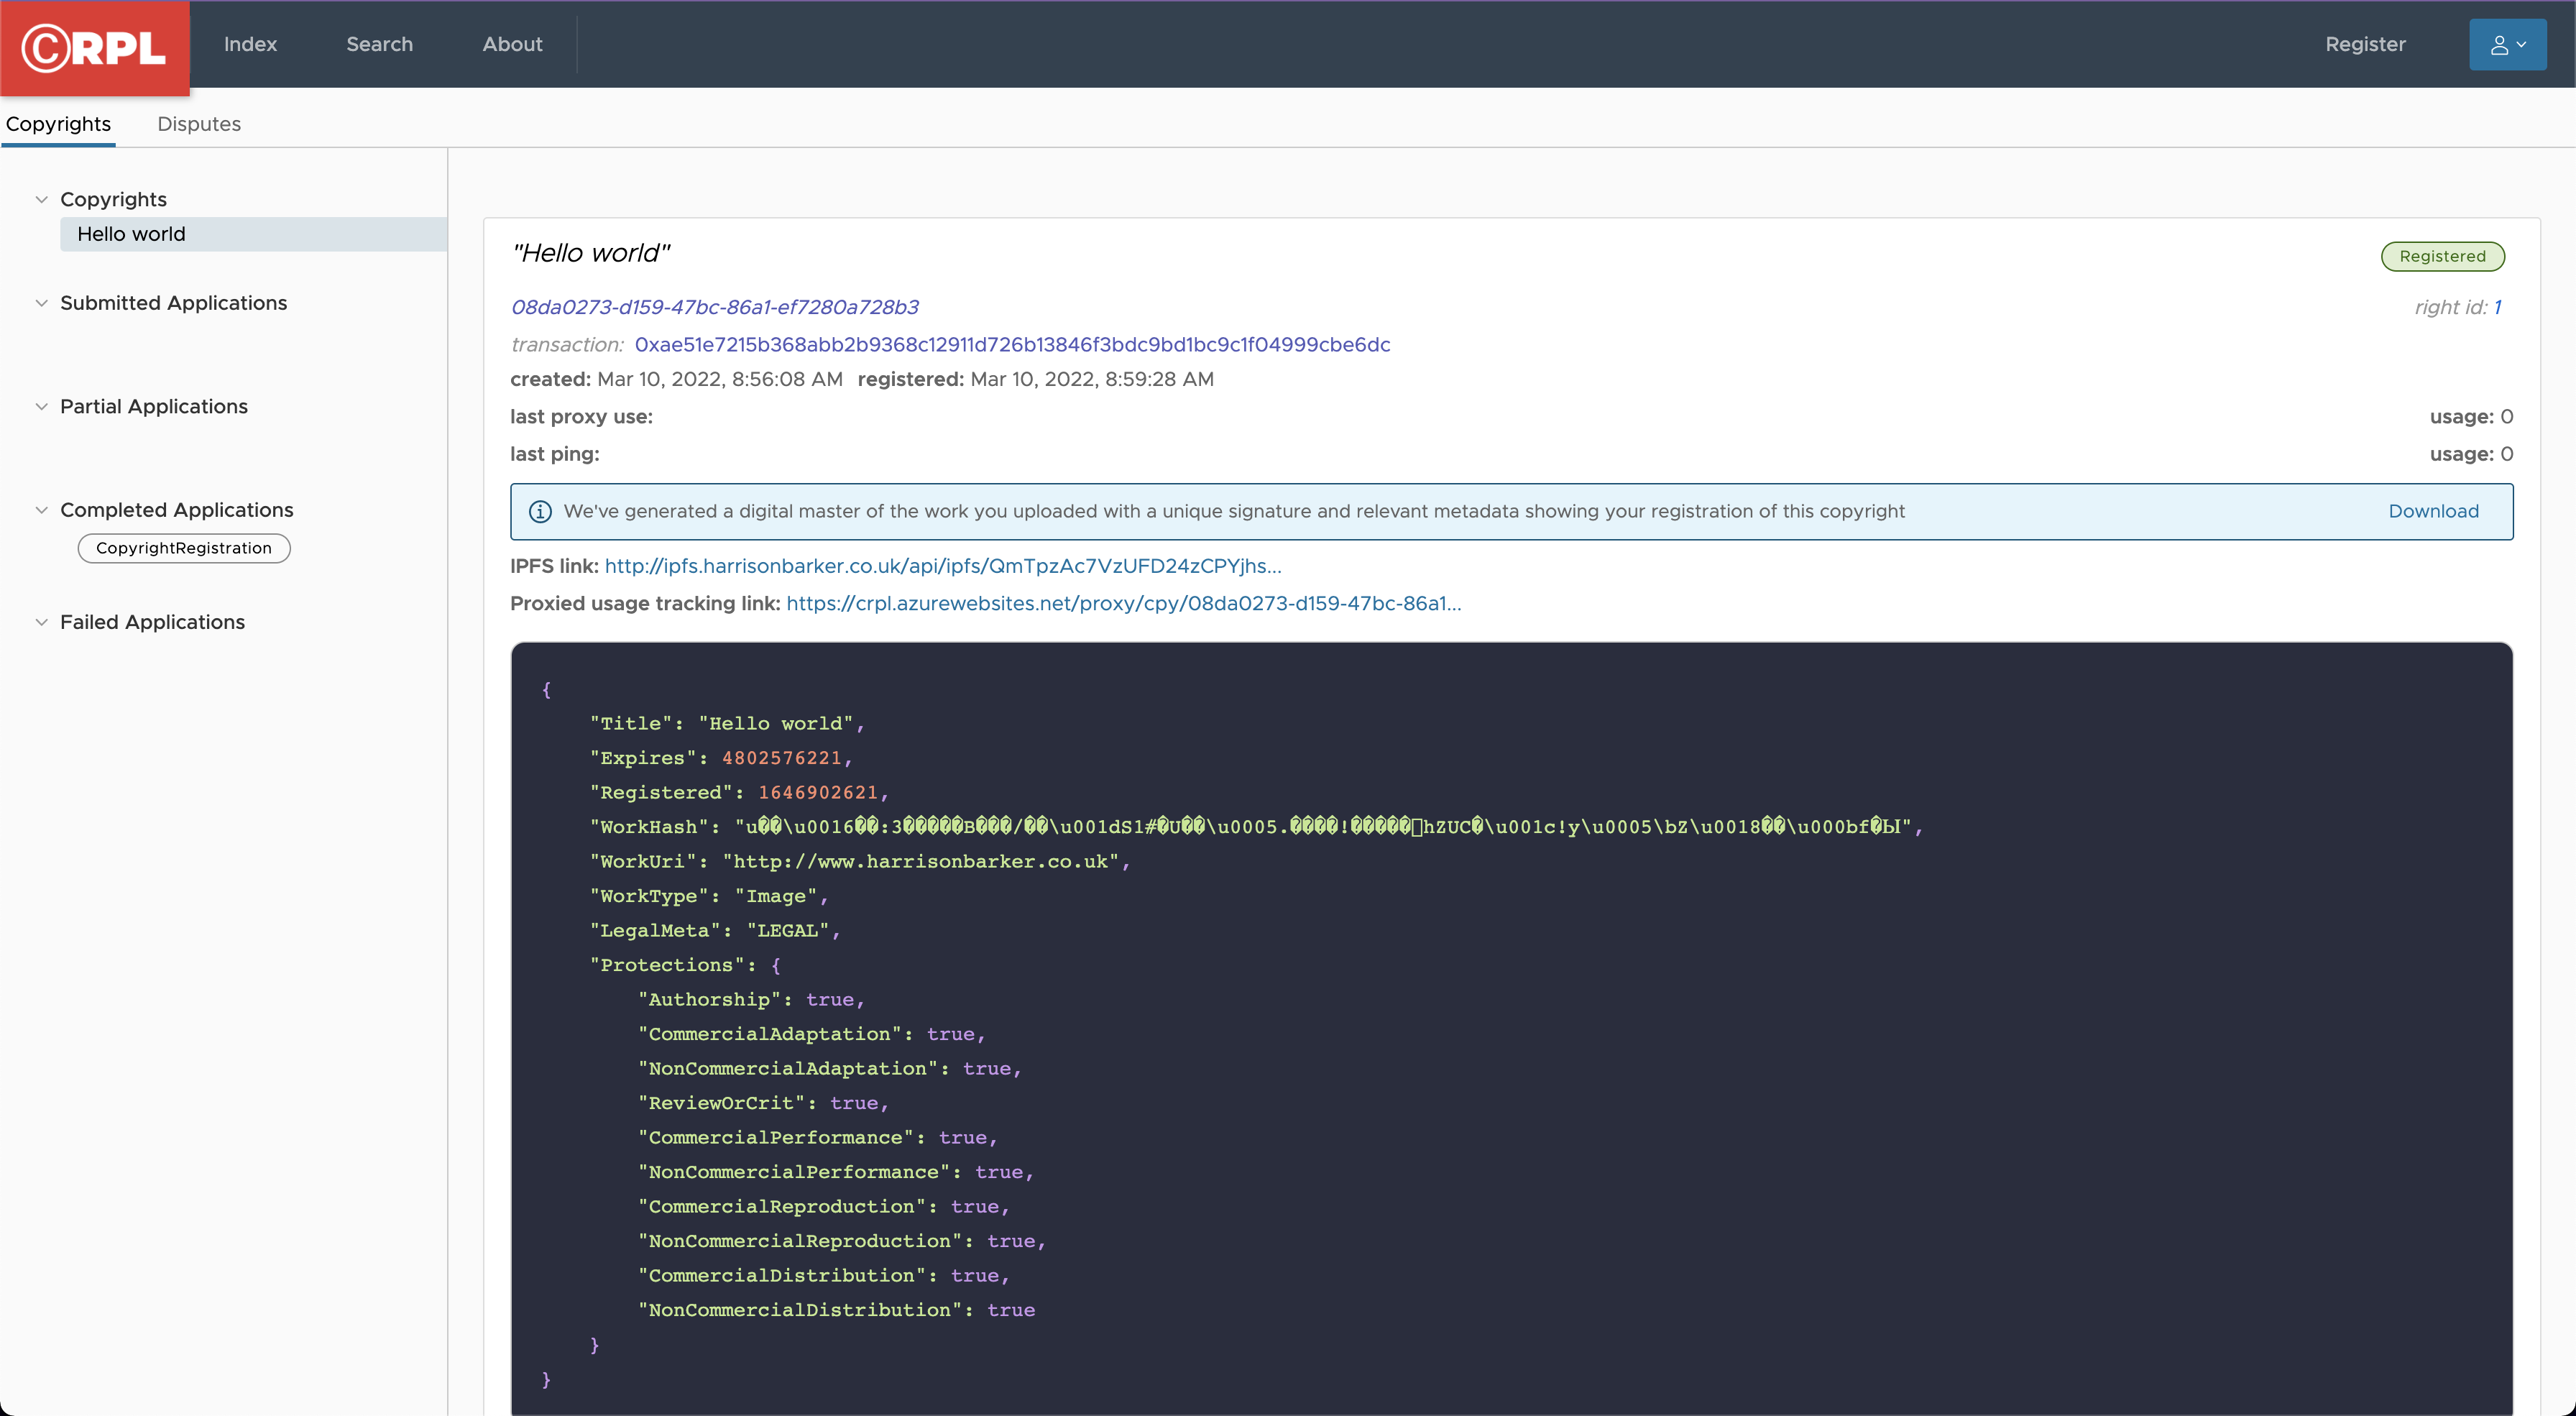
\includegraphics[width=\textwidth,height=0.5\textheight,keepaspectratio]{images/wireframe/dashboard-real}
\end{figure}

\begin{figure}[H]
\caption{Original register form wireframe}
\centering
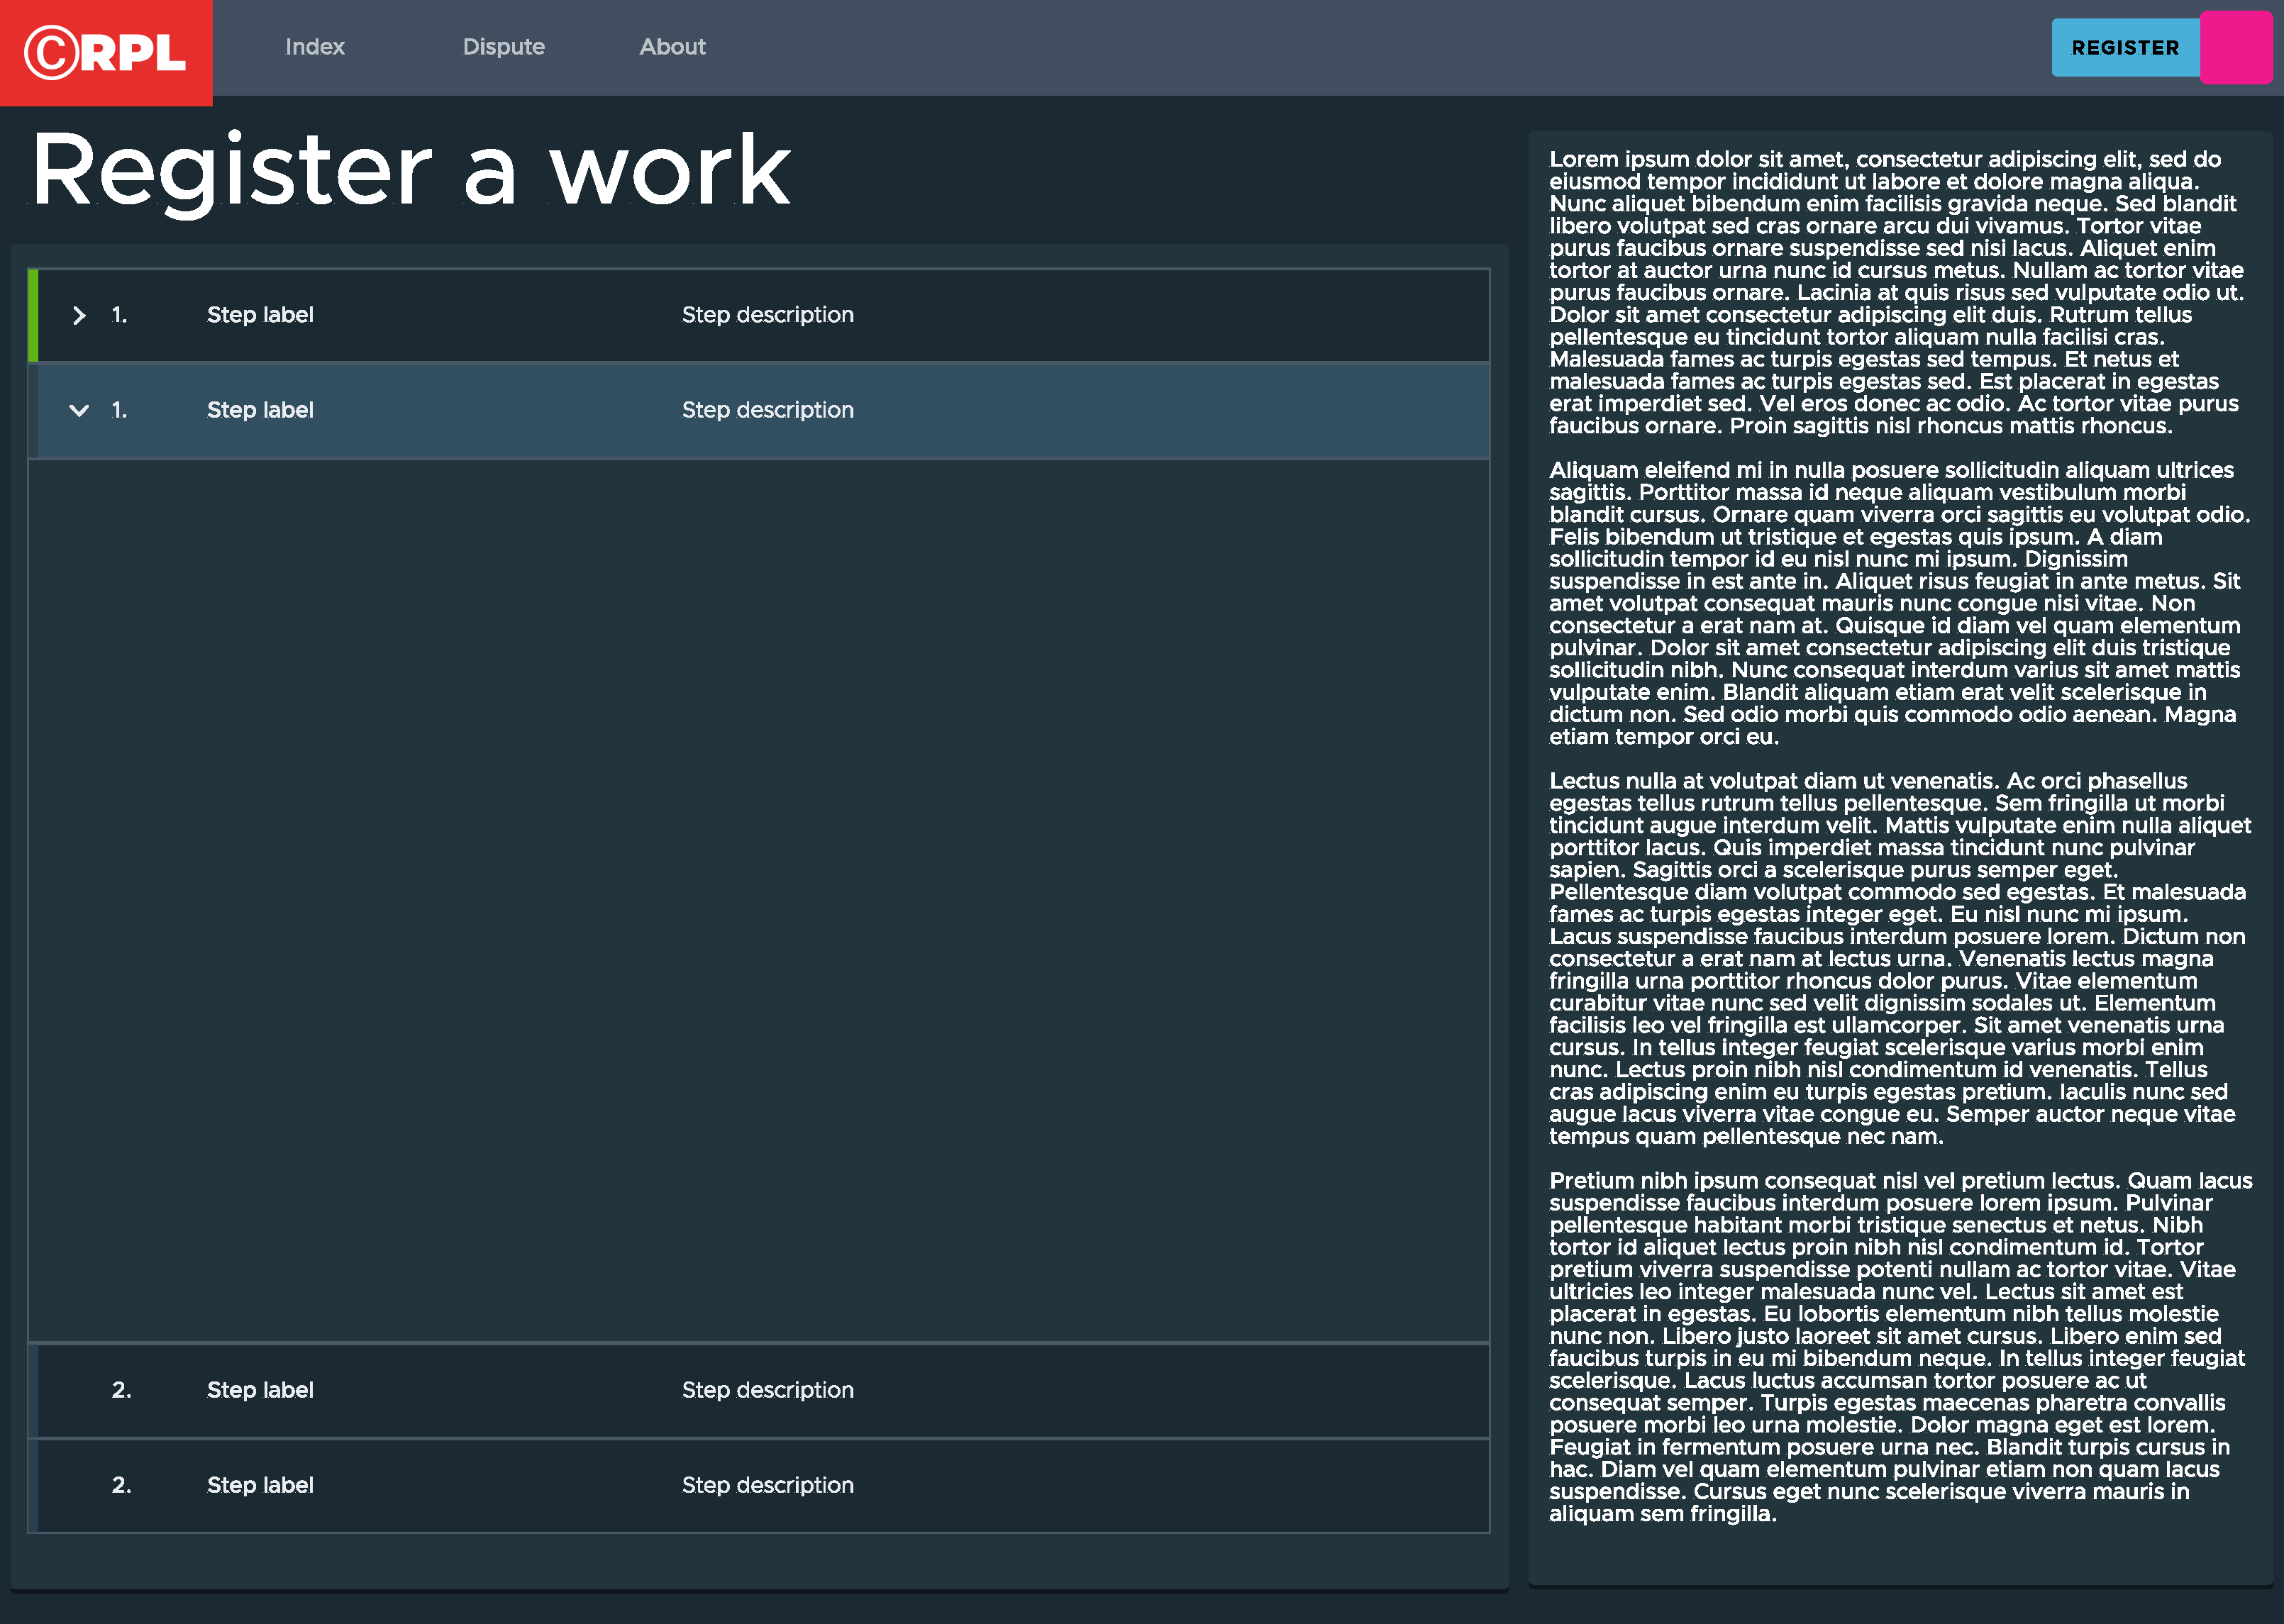
\includegraphics[width=\textwidth,height=0.5\textheight,keepaspectratio]{images/wireframe/Register}
\end{figure}

\begin{figure}[H]
\caption{Final register design}
\centering
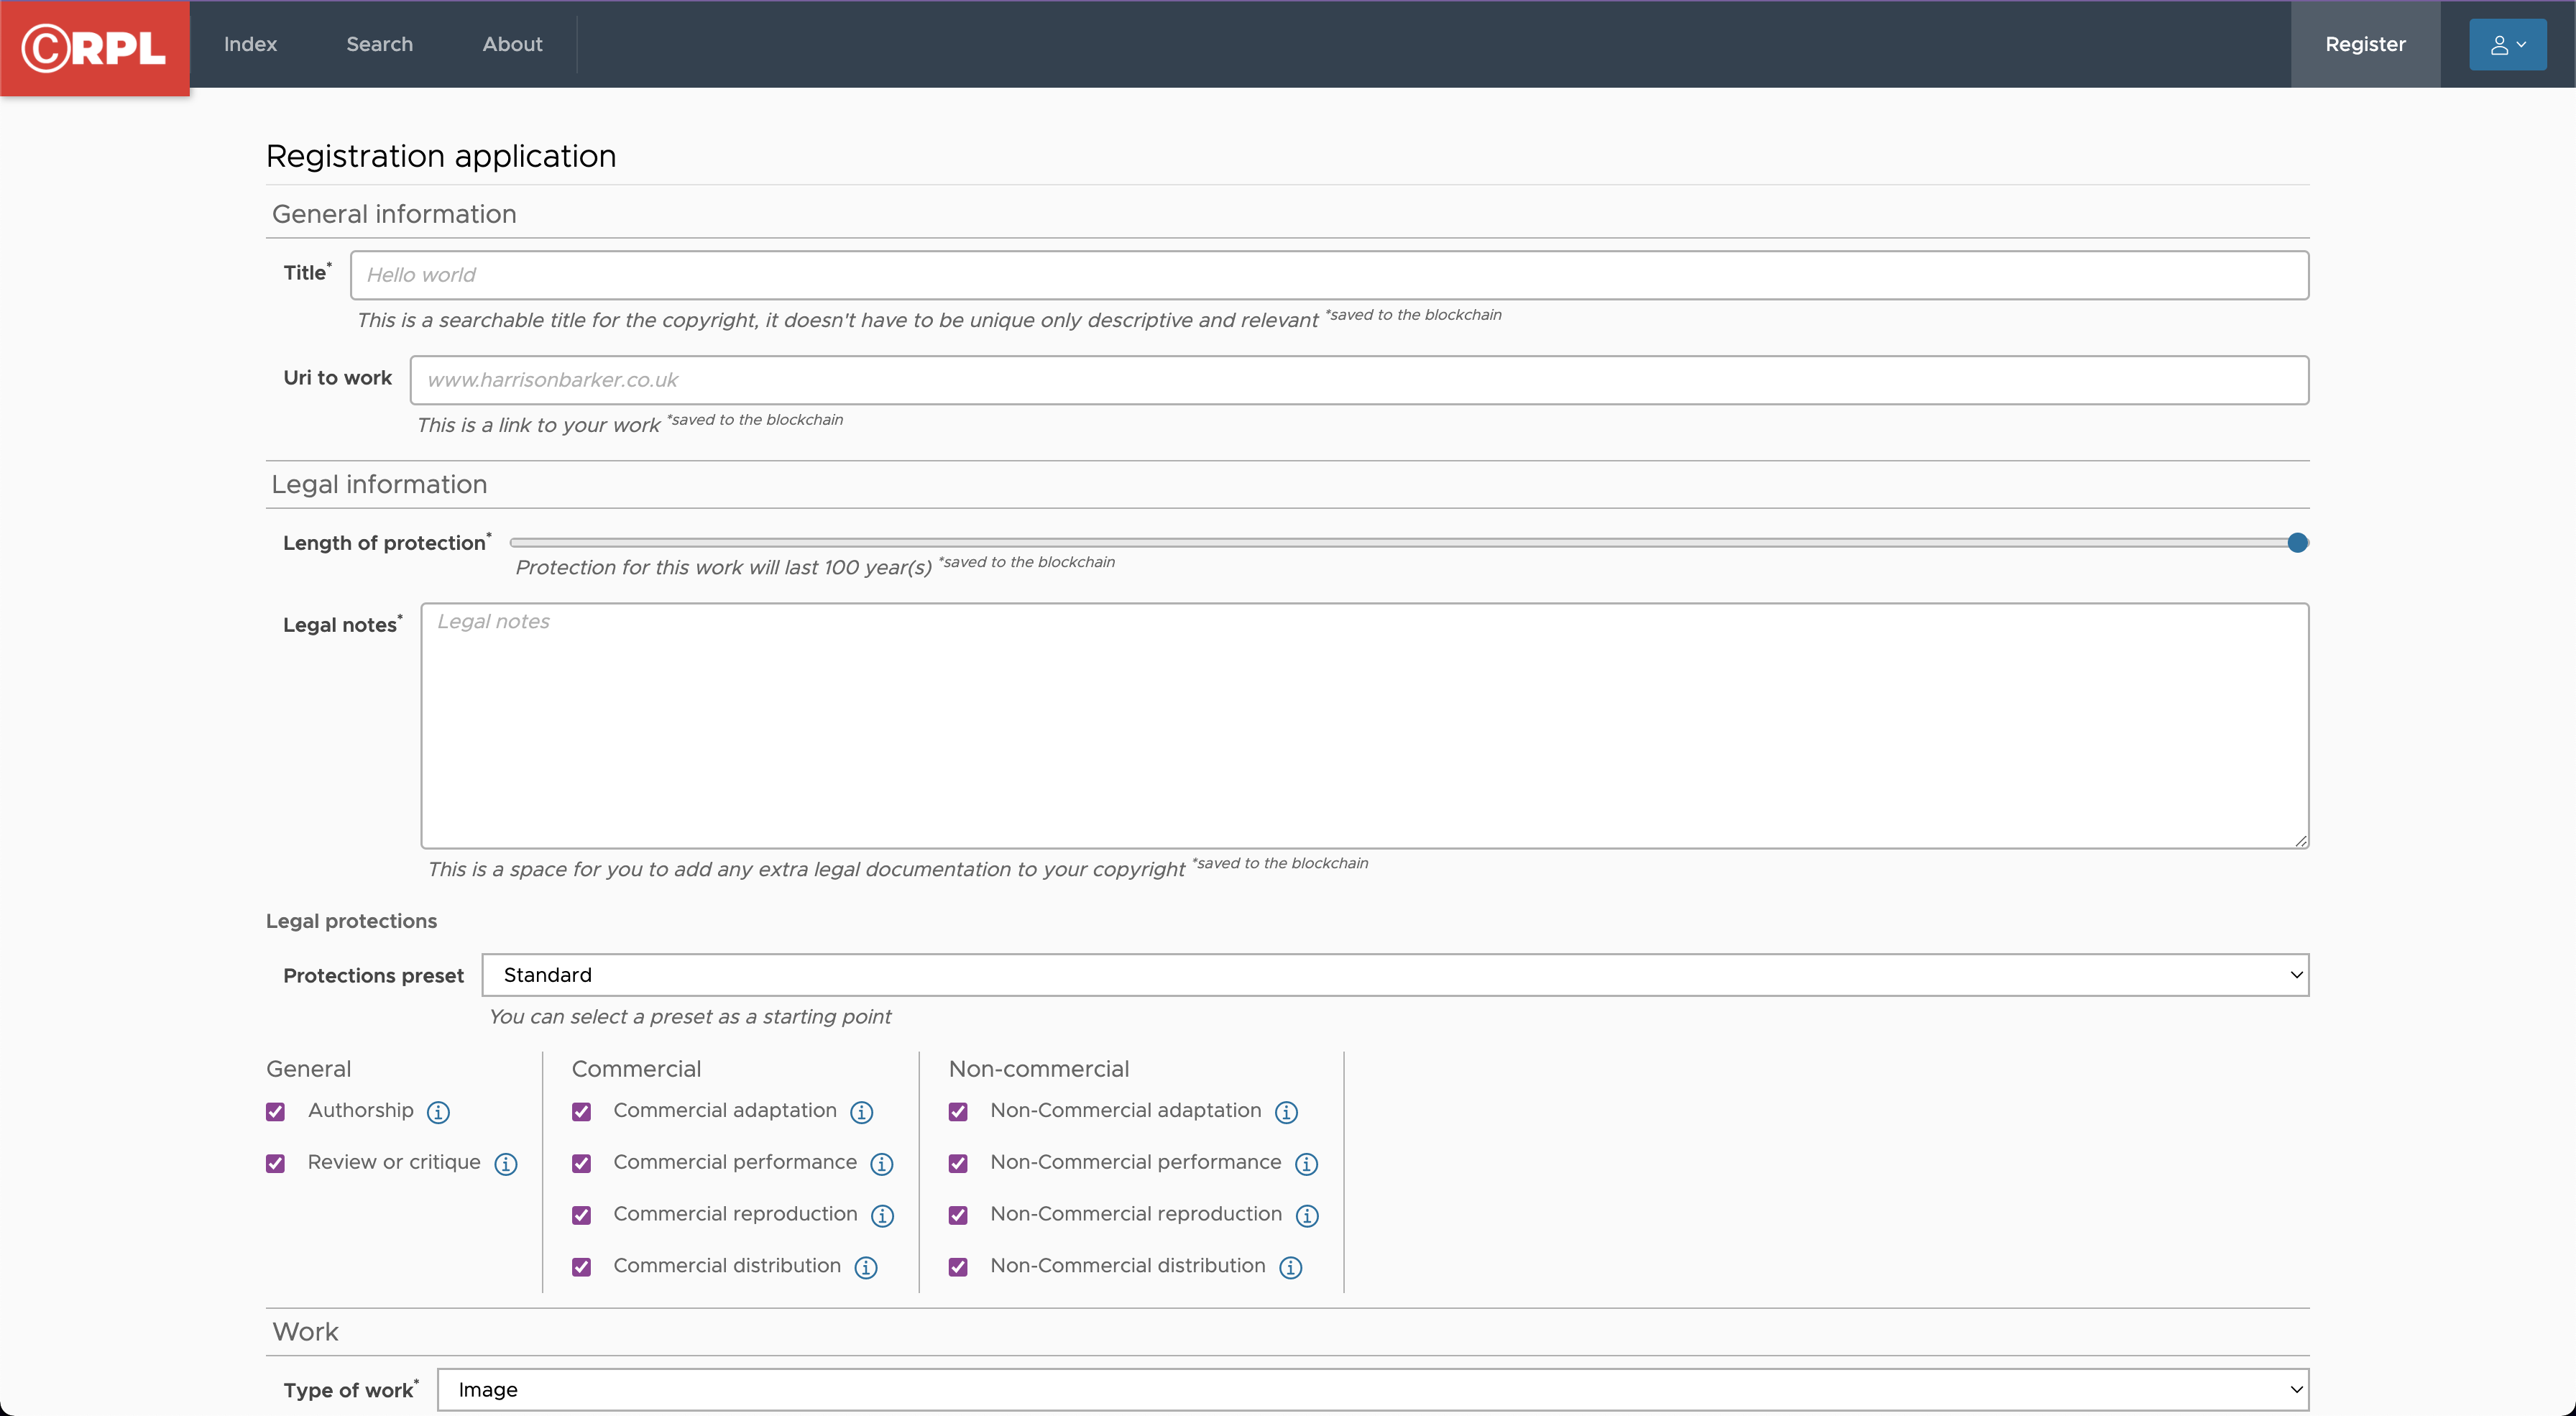
\includegraphics[width=\textwidth,height=0.5\textheight,keepaspectratio]{images/wireframe/register-real}
\end{figure}

\subsection{Architecture}
% TODO an overview of the system architecture design
TODO?

\subsection{Development process}

Development was split into four sprints, two larger sprints two weeks long to start development focusing on major core features essential for any success of the project: \keyword{smart contracts}, contract interaction, registration and restructure applications and user authentication. Followed up with two one week sprints focusing on secondary features and quality of life: disputes, search, synchronisation and account config.

\begin{figure}[H]
\hfil
\begin{tabular}{|p{0.2\textwidth}|p{0.3\textwidth}|p{0.3\textwidth}|p{0.2\textwidth}|}
\hline
Sprint & Start            & End              & Length  \\ \hline
1      & 19 January 2022  & 2 February 2022  & 2 weeks \\ \hline
2      & 4 February 2022  & 18 February 2022 & 2 weeks \\ \hline
3      & 20 February 2022 & 27 February 2022 & 1 week  \\ \hline
4      & 1 March 2022     & 8 March 2022     & 1 week  \\ \hline
\end{tabular}
\end{figure}